\documentclass{beamer}
\usepackage[italian]{babel}
\usepackage{algorithm}
\usepackage{algpseudocode}
\usepackage{float}
\usepackage{minted}
\usepackage{amsmath}
\usepackage{listings}
\usepackage{xcolor}
\usepackage{graphicx}
\usepackage{hyperref}
\usepackage[table]{xcolor}
\usepackage{amssymb}
\usepackage{csquotes}
\usepackage{hyperref}
\usepackage{algorithm}
\usepackage{algpseudocode}
\usepackage[table]{xcolor}
\usepackage{minted}
\usepackage{amsmath}
\usepackage{listings}
\usepackage{xcolor}
\usepackage{graphicx}
\usepackage{hyperref}
\usepackage{amssymb}

\DeclareMathOperator{\lcm}{lcm}

\title{Presentazione PHPC}
\author{Pierluigi Supino \and Rodolfo Diana \and Salvatore Di Gennaro}

\usetheme{default}
\begin{document}
\begin{frame}
    \titlepage
\end{frame}

\begin{frame}{Introduzione}
    \begin{itemize}
        \item Sviluppo di applicazione per il prodotto tra matrici su cluster multi-nodo e multi-GPU per nodo
        \item Il prodotto tra una matrice $\mathbf{A} \in \mathbb{R}^{m\times{k}}$ ed una seconda matrice $\mathbf{B} \in \mathbb{R}^{k\times{n}}$ è la matrice $\mathbf{C} \in \mathbb{R}^{m\times{n}}$ per cui: $$ \mathbf{C}_{i,j} = \sum_{l=0}^{\text{k}-1} \mathbf{A}_{i, l} \mathbf{B}_{l, j} $$
    \end{itemize}
\end{frame}

\begin{frame}{Implementazione}
    In ambiente multi-nodo e multi-GPU, il prodotto tra matrici viene scomposto in due sottoproblemi:
    \begin{enumerate}
        \item gestione a livello globale tra i processi, ovvero come suddividere le matrici e quali comunicazioni eseguire
        \item gestione a livello locale all'interno di ciascun nodo, ovvero come eseguire il prodotto sfruttando le GPU a disposizione
    \end{enumerate}
\end{frame}

\begin{frame}{Implementazione}{Processi}
    A livello di nodi:
    \begin{itemize}
        \item Scalable Universal Matrix Multiplication Algorithm (SUMMA)
        \item Algoritmo efficiente e flessibile per ogni numero di processi
    \end{itemize}
\end{frame}

\begin{frame}{Implementazione}{Processi}
    \begin{itemize}
        \item Si dispongono i processi in una griglia $r \times c$
        \item Si dividono le matrici $\mathbf{A}$ e $\mathbf{B}$ in $r \times \lcm(r,c)$ e $\lcm(r,c) \times c$ blocchi rispettivamente
        \item Si distribuiscono ciclicamente i blocchi delle matrici ai processi
    \end{itemize}
    \begin{figure}
        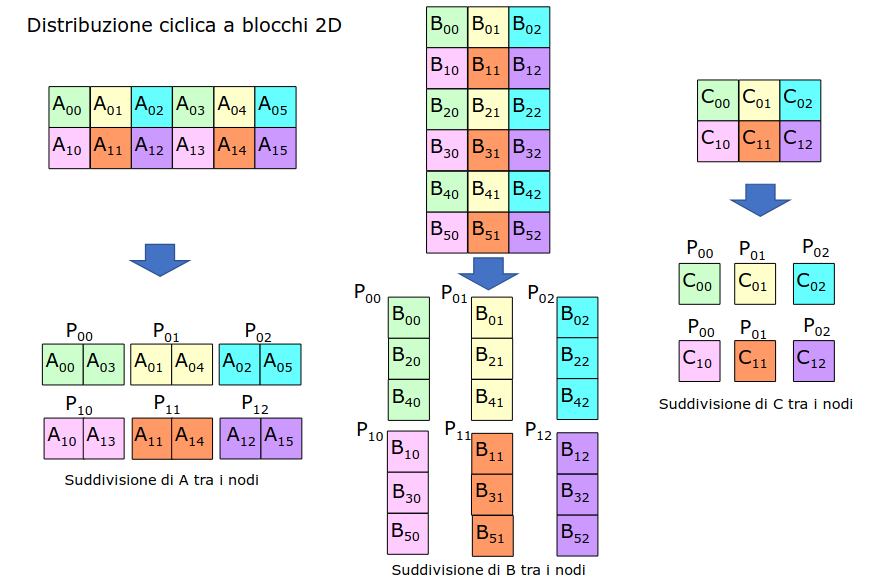
\includegraphics[width=0.55\linewidth]{imgs/summa.png}
        % \caption{Distribuzione SUMMA}
    \end{figure}
\end{frame}

\begin{frame}{Implementazione}{Processi}
    \begin{itemize}
        \item Per $\lcm(r,c)$ volte:
              \begin{enumerate}
                  \item Un processo invia il suo blocco di $\mathbf{A}$ alla propria riga
                  \item Un processo invia il suo blocco di $\mathbf{B}$ alla propria colonna
                  \item Viene sommato il prodotto parziale dei blocchi ricevuti
              \end{enumerate}
    \end{itemize}
    \begin{figure}
        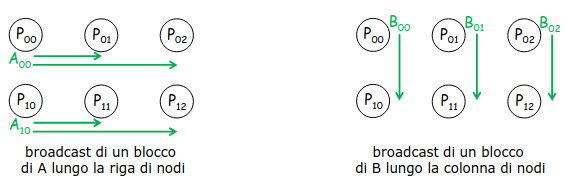
\includegraphics[width=0.75\linewidth]{imgs/broadcast_1.jpg}
        % \caption{Esempio di broadcast}
    \end{figure}
\end{frame}

\begin{frame}{Implementazione}{Processi}
    \begin{algorithm}[H]
        \caption{SUMMA for process $P_{i,j}$}
        \begin{algorithmic}
            \State $\mathbf{C}^{i,j} \gets 0$
            \State $l \gets \lcm(r,c)$
            \For{$k \gets 0$ \textbf{to} $l - 1$}
            \State $s \gets \bmod(k, r)$
            \State $t \gets \bmod(k, c)$
            \State process $P_{it}$ broadcasts $\mathbf{A}^{i,k}$ to its row
            \State process $P_{sj}$ broadcasts $\mathbf{B}^{k,j}$ to its column
            \State $\mathbf{C}^{i,j} \gets \mathbf{C}^{i,j} + \mathbf{A}^{i,k}\mathbf{B}^{k,j}$
            \EndFor
        \end{algorithmic}
    \end{algorithm}
\end{frame}

\begin{frame}{Implementazione}{Processi}
    \begin{itemize}
        \item Dati da inviare sparsi in memoria
              \begin{itemize}
                  \item Utilizzo di MPI\_Type\_vector per creare tipi personalizzati
              \end{itemize}
        \item Comunicazioni eseguite tramite MPI\_Bcast bloccanti
              \begin{itemize}
                  \item Nessun vantaggio riscontrato nell'utilizzo di versioni asincrone
              \end{itemize}
    \end{itemize}

    \begin{figure}[h]
        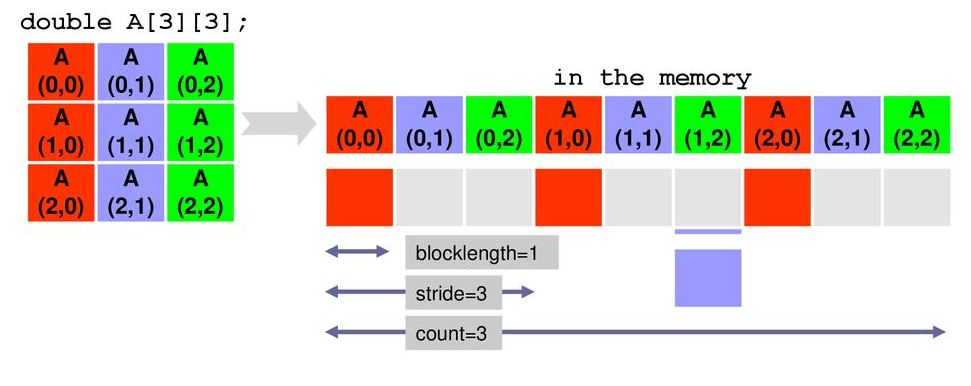
\includegraphics[width=0.7\linewidth]{imgs/mpi_type_vector.png}
        % \caption{Distribuzione dei dati}
    \end{figure}
\end{frame}

\begin{frame}{Implementazione}{Processi}
    \begin{itemize}
        \item Semplificazioni e assunzioni effettuate:
              \begin{itemize}
                  \item solo matrici quadrate $n \times n$, con $n$ multiplo di $\lcm(r,c)$
                  \item matrici di input di ogni processo come array contigui \textit{row-major} contenenti già i dati necessari
                  \item gestione degli errori quasi assente per evitare overhead
              \end{itemize}
    \end{itemize}
\end{frame}

\begin{frame}{Implementazione}{GPU}
    \begin{itemize}
        \item Si passa al calcolo effettivo delle (sotto)matrici
        \item Potenzialmente più GPU per processo
        \item Come parallelizzare il lavoro?
              \begin{enumerate}
                  \item Evitare conflitti di memoria da serializzare
                  \item Avviare contemporaneamente sui diversi device (senza attendere)
              \end{enumerate}
    \end{itemize}
\end{frame}

\begin{frame}{Implementazione}{GPU}
    \begin{enumerate}
        \item Evitare conflitti di memoria da serializzare
    \end{enumerate}
    \medskip

    \begin{itemize}
        \item Evitare scritture concorrenti su $\mathbf{C}$
              \begin{itemize}
                  \item $\mathbf{A}$ e $\mathbf{B}$ solo in lettura quindi nessun problema
              \end{itemize}
        \item Partizionare $\mathbf{C}$ in blocchi separati gestiti ognuno da una GPU
              \begin{itemize}
                  \item Suddivisione in colonne per semplicità
                  \item $\mathbf{C}^i = \mathbf{A} \times  \mathbf{B}^i$
              \end{itemize}
    \end{itemize}

    \begin{figure}[h]
        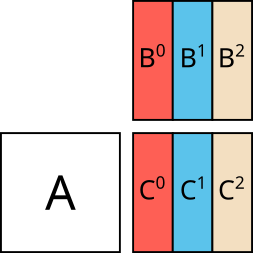
\includegraphics[width=0.25\linewidth]{imgs/gpu.png}
    \end{figure}
\end{frame}

\begin{frame}{Implementazione}{GPU}
    \begin{enumerate}
        \item[2.] Avviare contemporaneamente su diversi device (senza attendere)
    \end{enumerate}
    \medskip

    \begin{itemize}
        \item Pattern fork-join con ogni thread che gestisce una GPU...
        \item ...oppure \alert{Utilizzo dei metodi async e degli stream di CUDA}
              \begin{itemize}
                  \item Stream: coda di operazioni da gestire in sequenza
                  \item Host avvia lavoro su stream diversi per ogni GPU
              \end{itemize}
    \end{itemize}

    \begin{figure}[h]
        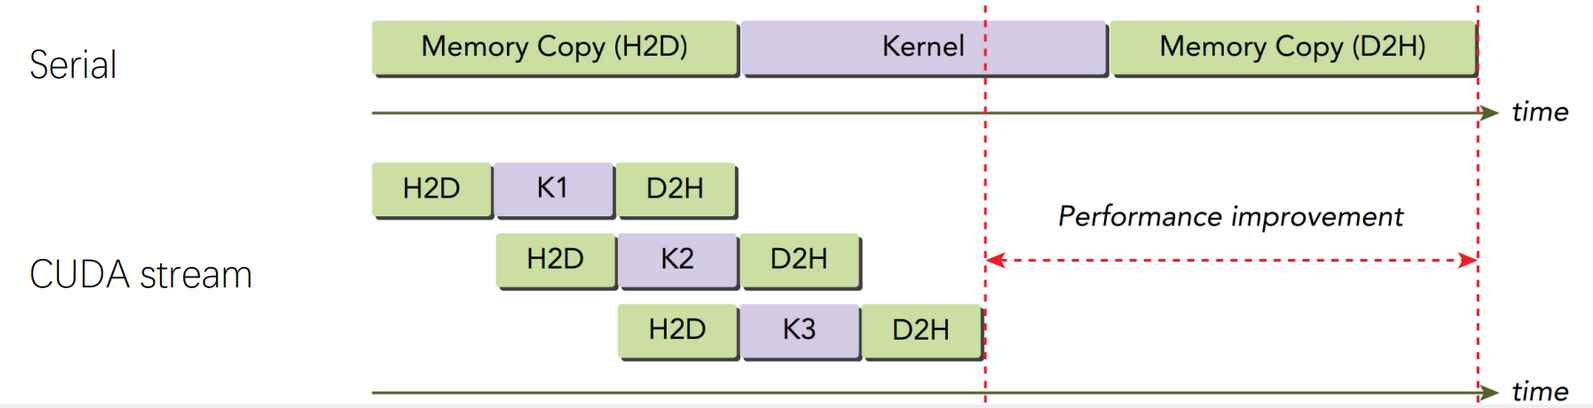
\includegraphics[width=0.8\linewidth]{imgs/cuda_stream.png}
    \end{figure}
\end{frame}

\begin{frame}{Implementazione}{Processi}
    \begin{algorithm}[H]
        \caption{MultiGPU}
        \begin{algorithmic}
            \For{$i \gets 0$ \textbf{to} gpu count}
            \State set device to $i$
            \State create stream $i$
            \State async copy $\mathbf{A}, \mathbf{B}^i, \mathbf{C}^i$ from host to device on stream $i$
            \State async execute $\mathbf{C}^{i} \gets \mathbf{C}^{i} + \mathbf{A}\mathbf{B}^{i}$ on stream $i$
            \State async copy $\mathbf{A}, \mathbf{B}^i, \mathbf{C}^i$ from device to host on stream $i$
            \EndFor

            \For{$i \gets 0$ \textbf{to} gpu count}
            \State wait stream $i$
            \State destroy stream $i$
            \EndFor
        \end{algorithmic}
    \end{algorithm}
\end{frame}

\begin{frame}{Implementazione}{GPU - cuBLAS}
    \begin{itemize}
        \item Problema del prodotto matriciale già ampiamente discusso
        \item Numerose librerie disponibili: \alert{cuBLAS}
              \begin{itemize}
                  \item implementazione ottimizzata per GPU NVIDIA delle specifiche BLAS
                        \begin{itemize}
                            \item Per compatibilità con Fortran si aspetta ordine column-major
                            \item Basta calcolare $\mathbf{C}^T=(\mathbf{B}\mathbf{A})^T$
                        \end{itemize}
                  \item \alert{cuBLASXt}: estensione per ambienti multi-GPU
              \end{itemize}
    \end{itemize}
\end{frame}

\begin{frame}{Implementazione}{Kernel 1}
    \begin{itemize}
        \item Per implementare la moltiplicazione tra matrici in CUDA possiamo:
              \begin{itemize}
                  \item Mappare i thread della griglia agli elementi della matrice di output in modo che ognugno sia responsabile del calcolo del singolo elemento.
                  \item Gli indici dell'elemento che ogni thread dovrà calcolare saranno:
                        \begin{itemize}
                            \item \textit{row = blockIdx.y × blockDim.y + threadIdx.y}
                            \item \textit{col = blockIdx.x × blockDim.x + threadIdx.x}
                        \end{itemize}
              \end{itemize}
    \end{itemize}
\end{frame}

\begin{frame}{Implementazione}{Kernel 1}
    \begin{algorithm}[H]
        \caption{Matrix Multiplication Kernel 1}
        \begin{algorithmic}[1]
            \State $\texttt{row} \gets \texttt{blockIdx.y} \cdot \texttt{blockDim.y} + \texttt{threadIdx.y}$
            \State $\texttt{col} \gets \texttt{blockIdx.x} \cdot \texttt{blockDim.x} + \texttt{threadIdx.x}$
            \If{$\texttt{row} < \texttt{Width}$ \textbf{and} $\texttt{col} < \texttt{Width}$}
            \State $\texttt{Pval} \gets 0$
            \For{$k \gets 0$ \textbf{to} $\texttt{Width} - 1$}
            \State $\texttt{Pval} \gets \texttt{Pval} + M[\texttt{row} \cdot \texttt{Width} + k] \cdot N[k \cdot \texttt{Width} + \texttt{col}]$
            \EndFor
            \State $P[\texttt{row} \cdot \texttt{Width} + \texttt{col}] \gets \texttt{Pval}$
            \EndIf
        \end{algorithmic}
    \end{algorithm}
\end{frame}

\begin{frame}{Implementazione}{Kernel 1}
    \begin{figure}[H]
        \centering
        \begin{minipage}{0.48\textwidth}
            \centering
            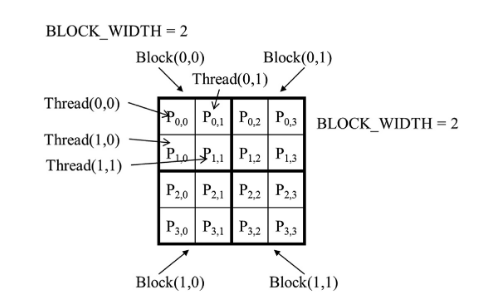
\includegraphics[width=\linewidth]{imgs/matrix_division.png}
            \caption{Figura 1: Divisione degli elementi in una griglia 2x2 con blocchi 2x2}
        \end{minipage}
        \hfill
        \begin{minipage}{0.48\textwidth}
            \centering
            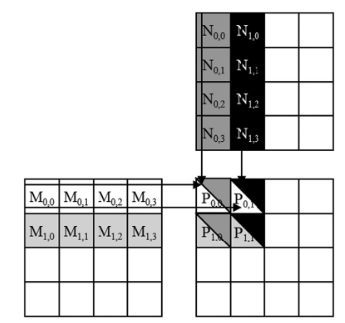
\includegraphics[width=\linewidth]{imgs/execution1.png}
            \caption{Figura 2: Esempio di calcolo}
        \end{minipage}
    \end{figure}
\end{frame}

\begin{frame}{Implementazione}{Kernel 1}
    \begin{itemize}
        \item Ampi margini di miglioramento rispetto alla memoria
              \begin{itemize}
                  \item La memoria globale è grande ma lenta
                  \item La memoria condivisa è piccola ma veloce
              \end{itemize}
    \end{itemize}
    \begin{figure}[H]
        \centering
        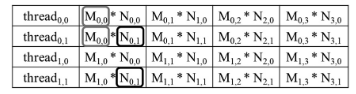
\includegraphics[width=0.7\textwidth]{imgs/memory_access.png}
    \end{figure}
    \begin{itemize}
        \item Idea: Partizionare i dati in sottoinsiemi chiamati tiles, in modo tale che ognuna di essa entri nella memoria condivisa. Tutti i thread collaboreranno al caricamento delle tiles in memoria condivisa prima della computazione. Stiamo riducendo gli accessi alla memoria globale di un fattore $\frac{1}{width}$
    \end{itemize}
\end{frame}

\begin{frame}{Implementazione}{Kernel 2}
    \begin{figure}[H]
        \centering
        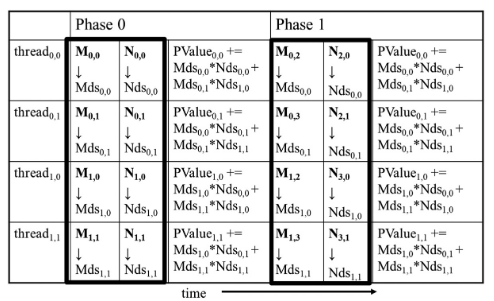
\includegraphics[width=0.7\textwidth]{imgs/memory_access1.png}
        \caption{Figura 3: Accessi alla memoria nuovo approccio}
    \end{figure}
\end{frame}

\begin{frame}{Implementazione}{Kernel 2}
    \begin{algorithm}[H]
        \caption{Tiled Matrix Multiplication Kernel 2}
        \begin{algorithmic}[1]
            \State \texttt{Pval} $\gets$ 0
            \For{$ph \gets 0$ \textbf{to} $\texttt{Width} / \texttt{TILE\_WIDTH} - 1$}
            \State $M_{ds}[ty][tx] \gets M[Row \cdot Width + ph \cdot TILE\_WIDTH + tx]$
            \State $N_{ds}[ty][tx] \gets N[(ph \cdot TILE\_WIDTH + ty) \cdot Width + Col]$
            \State \texttt{syncthreads()}
            \For{$k \gets 0$ \textbf{to} \texttt{TILE\_WIDTH} - 1}
            \State \texttt{Pval} $\gets$ \texttt{Pval} $+$ $M_{ds}[ty][k] \cdot N_{ds}[k][tx]$
            \EndFor
            \State \texttt{syncthreads()}
            \EndFor
            \State $P[Row \cdot Width + Col] \gets$ \texttt{Pval}
        \end{algorithmic}
    \end{algorithm}
\end{frame}

\begin{frame}{Implementazione}{Kernel 2}
    \begin{algorithm}[H]
        \scriptsize
        \caption{Tiled Matrix Multiplication Kernel 2 con padding}
        \begin{algorithmic}[1]
            \State $Pval \gets 0$
            \For{$ph \gets 0$ \textbf{to} $\lceil W/T \rceil -1$}
            \State $M_{ds}[ty][tx] \gets (Row<W~\&\&~ph\cdot T+tx<W)~?~M[Row\cdot W + ph\cdot T + tx]~:~0$
            \State $N_{ds}[ty][tx] \gets (ph\cdot T+ty<W~\&\&~Col<W)~?~N[(ph\cdot T+ty)\cdot W + Col]~:~0$
            \State \texttt{syncthreads()}
            \For{$k \gets 0$ \textbf{to} $T-1$}
            \State $Pval \mathrel{+}= M_{ds}[ty][k] \cdot N_{ds}[k][tx]$
            \EndFor
            \State \texttt{syncthreads()}
            \EndFor
            \If{$Row < W~\&\&~Col < W$}
            \State $P[Row\cdot W + Col] \gets Pval$
            \EndIf
        \end{algorithmic}
    \end{algorithm}
\end{frame}

\begin{frame}{Implementazione}{Kernel 3}
    \begin{itemize}
        \item TODO
    \end{itemize}
\end{frame}

\begin{frame}
    \centering \Huge
    Analisi
\end{frame}

\begin{frame}{Analisi}
    \begin{itemize}
        \item Sono stati riscontrati problemi con il cluster
              \begin{itemize}
                  \item SEGFAULT della versione installata di OpenMPI
              \end{itemize}
        \item Non è stato possibile analizzare correttamente l'esecuzione
        \item Qualche risultato ottenuto da esecuzione su macchina locale
              \begin{itemize}
                  \item Non rappresentativo delle vere performance
                  \item Nessuna analisi da Nsight Compute
                        %   \item NVIDIA RTX 4060 % TODO: spec

                  \item CPU AMD Ryzen 5 7600
                  \item GPU NVIDIA GTX 1050Ti
                  \item 32 GB di RAM
              \end{itemize}
    \end{itemize}
\end{frame}

\begin{frame}{Analisi}{Test - 1a}
    \begin{enumerate}
        \item[1a] Aumentando le dimensioni della matrice, a parità di processi (4) e thread (1024)
    \end{enumerate}

    \begin{figure}[H]
        \centering
        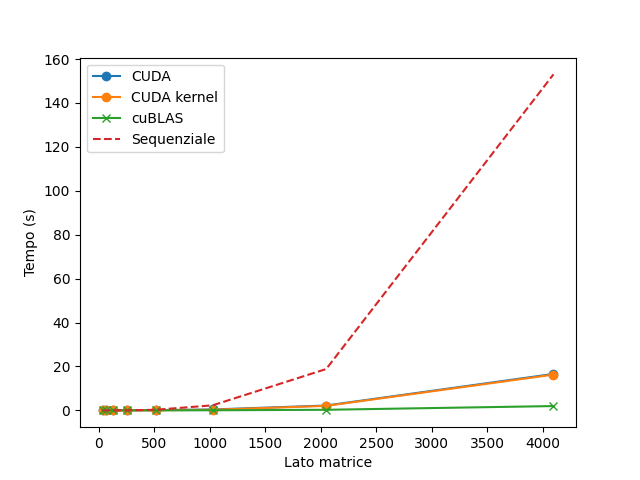
\includegraphics[width=0.6\textwidth]{./imgs/graphs/caso_0.png}
    \end{figure}
\end{frame}

\begin{frame}{Analisi}{Test - 1a}
    \begin{figure}[H]
        \centering
        \begin{minipage}{0.49\textwidth}
            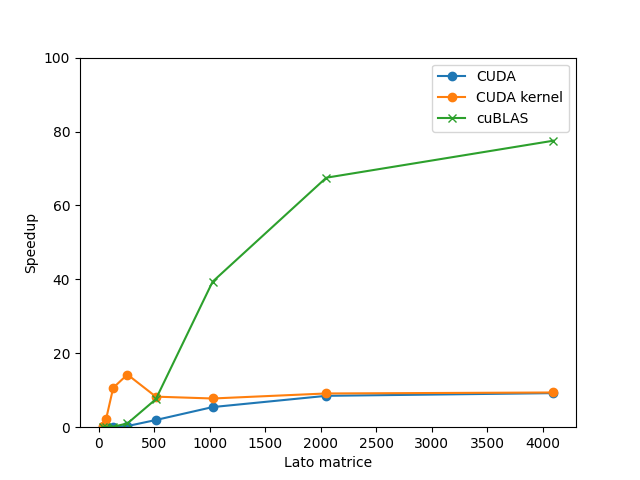
\includegraphics[width=\textwidth]{./imgs/graphs/caso_0_speedup.png}
        \end{minipage}
        \begin{minipage}{0.49\textwidth}
            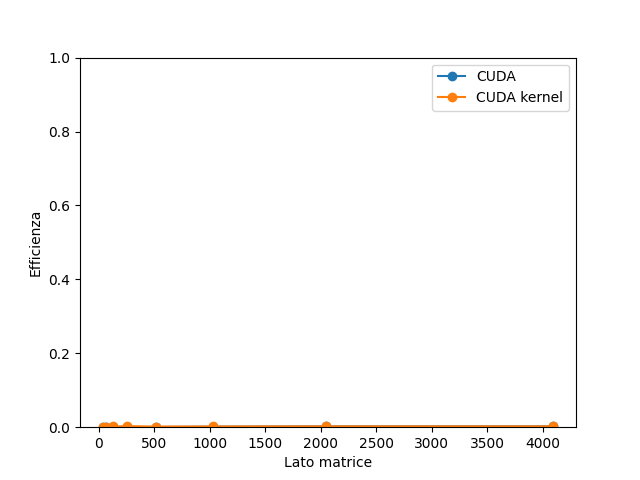
\includegraphics[width=\textwidth]{./imgs/graphs/caso_0_efficiency.png}
        \end{minipage}
    \end{figure}
\end{frame}

\begin{frame}{Analisi}{Test - 1b}
    \begin{enumerate}
        \item[1b] Aumentando i processi, a parità di thread (1024) e dimensioni della matrice ($2048 \times 2048$)
    \end{enumerate}

    \begin{figure}[H]
        \centering
        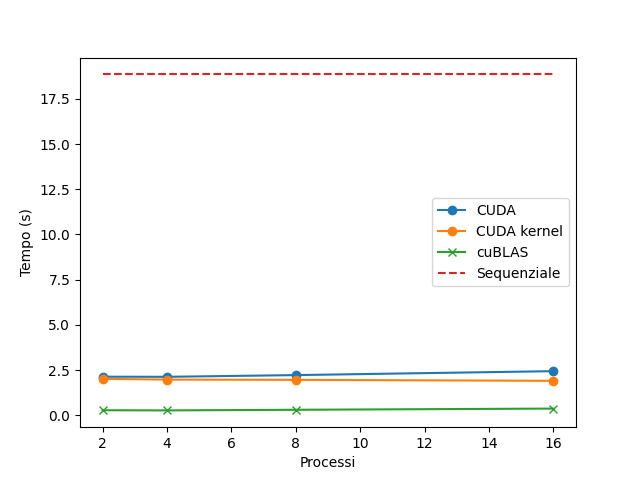
\includegraphics[width=0.6\textwidth]{./imgs/graphs/caso_a1.png}
    \end{figure}
\end{frame}

\begin{frame}{Analisi}{Test - 1b}
    \begin{figure}[H]
        \centering
        \begin{minipage}{0.49\textwidth}
            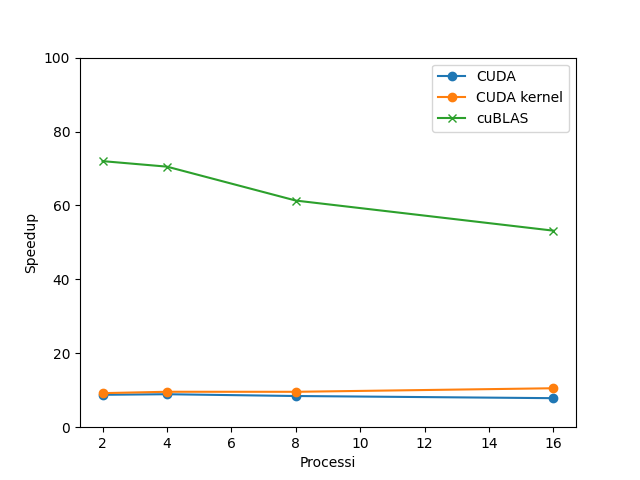
\includegraphics[width=\textwidth]{./imgs/graphs/caso_a1_speedup.png}
        \end{minipage}
        \begin{minipage}{0.49\textwidth}
            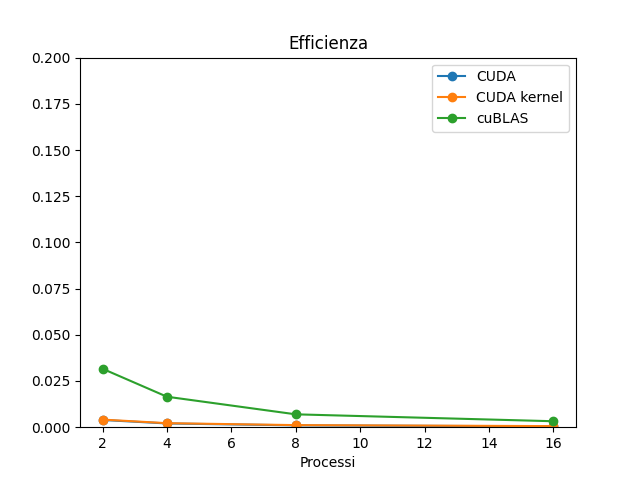
\includegraphics[width=\textwidth]{./imgs/graphs/caso_a1_efficiency.png}
        \end{minipage}
    \end{figure}
\end{frame}

\begin{frame}{Analisi}{Test - 1c}
    \begin{enumerate}
        \item[1c] Aumentando i thread, a parità di processi (4) e dimensioni della matrice ($2048 \times 2048$)
    \end{enumerate}

    \begin{figure}[H]
        \centering
        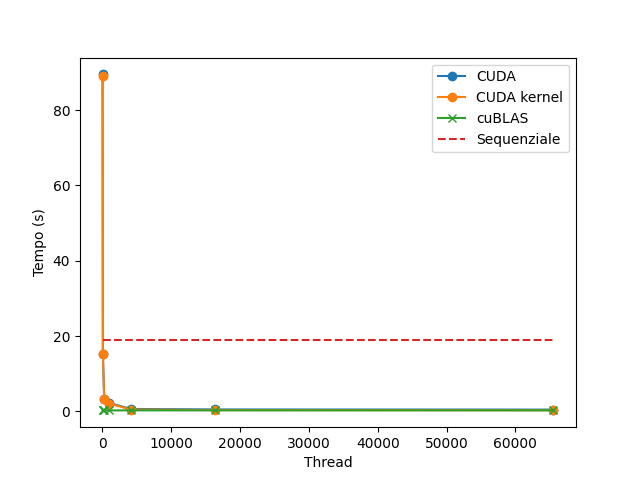
\includegraphics[width=0.6\textwidth]{./imgs/graphs/caso_a2.png}
    \end{figure}
\end{frame}

\begin{frame}{Analisi}{Test - 1c}
    \begin{figure}[H]
        \centering
        \begin{minipage}{0.49\textwidth}
            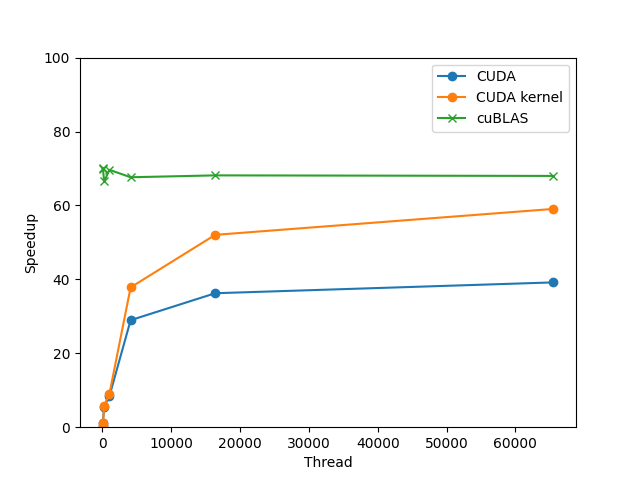
\includegraphics[width=\textwidth]{./imgs/graphs/caso_a2_speedup.png}
        \end{minipage}
        \begin{minipage}{0.49\textwidth}
            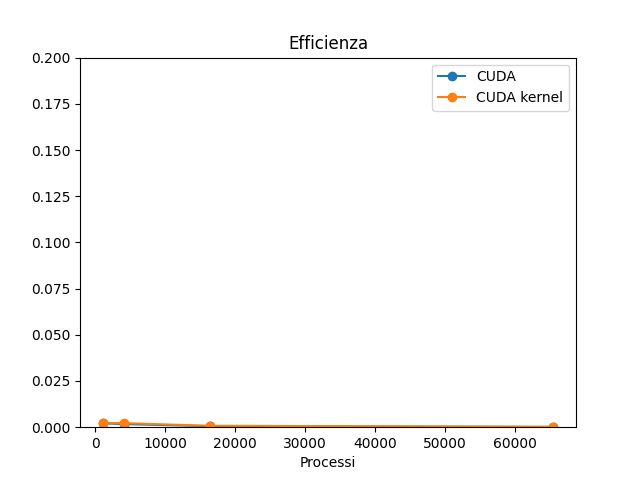
\includegraphics[width=\textwidth]{./imgs/graphs/caso_a2_efficiency.png}
        \end{minipage}
    \end{figure}
\end{frame}

\begin{frame}{Analisi}{Test - 2}
    \begin{enumerate}
        \item[2.] Aumentando i processi, a parità di thread ($1024 \times 1024$) e dimensione del problema \textbf{per processo} ($1024 \times 1024$)
    \end{enumerate}

    \begin{figure}[H]
        \centering
        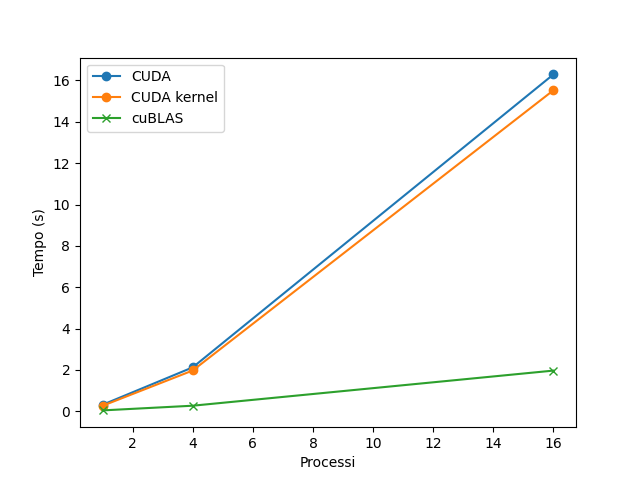
\includegraphics[width=0.6\textwidth]{./imgs/graphs/caso_b.png}
    \end{figure}
\end{frame}

\begin{frame}{Analisi}{Test - 2}
    \begin{figure}[H]
        \centering
        \begin{minipage}{0.49\textwidth}
            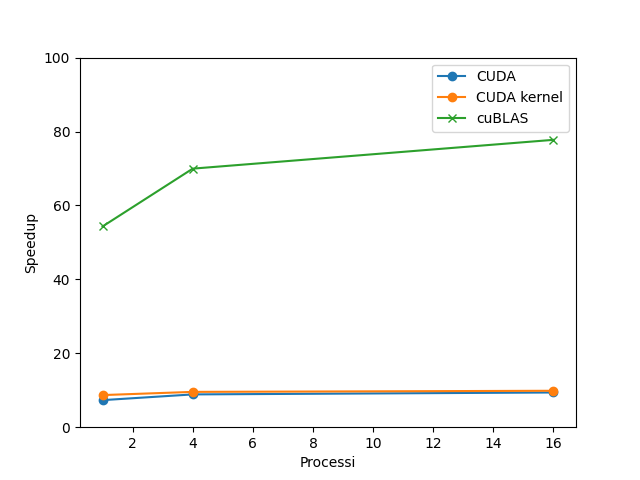
\includegraphics[width=\textwidth]{./imgs/graphs/caso_b_speedup.png}
        \end{minipage}
        \begin{minipage}{0.49\textwidth}
            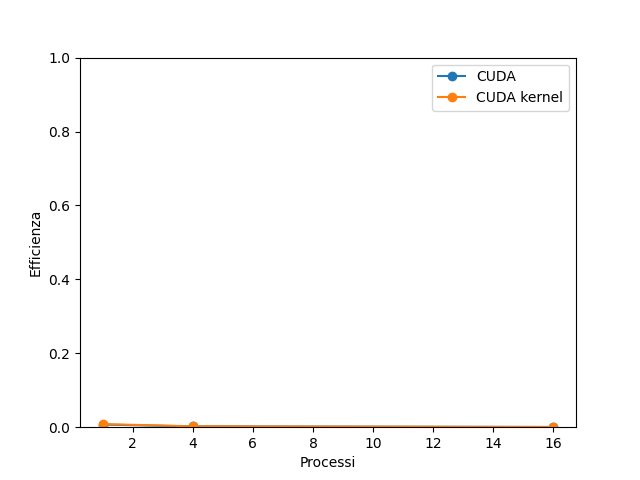
\includegraphics[width=\textwidth]{./imgs/graphs/caso_b_efficiency.png}
        \end{minipage}
    \end{figure}
\end{frame}

\begin{frame}{Analisi}{Test - 3}
    \begin{enumerate}
        \item[3.] Aumentando i thread, a parità di processi (4) e dimensione del problema \textbf{per thread}
    \end{enumerate}

    \begin{figure}[H]
        \centering
        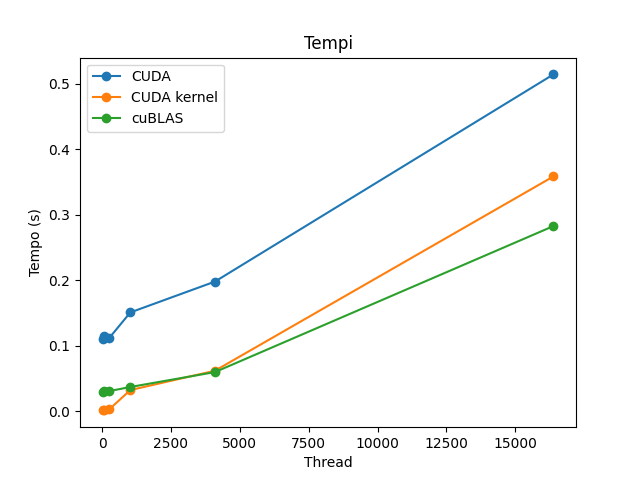
\includegraphics[width=0.6\textwidth]{./imgs/graphs/caso_c.png}
    \end{figure}
\end{frame}

\begin{frame}{Analisi}{Test - 3}
    \begin{figure}[H]
        \centering
        \begin{minipage}{0.49\textwidth}
            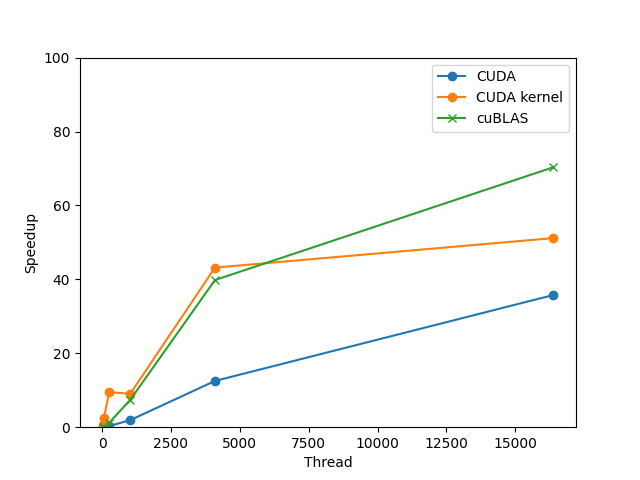
\includegraphics[width=\textwidth]{./imgs/graphs/caso_c_speedup.png}
        \end{minipage}
        \begin{minipage}{0.49\textwidth}
            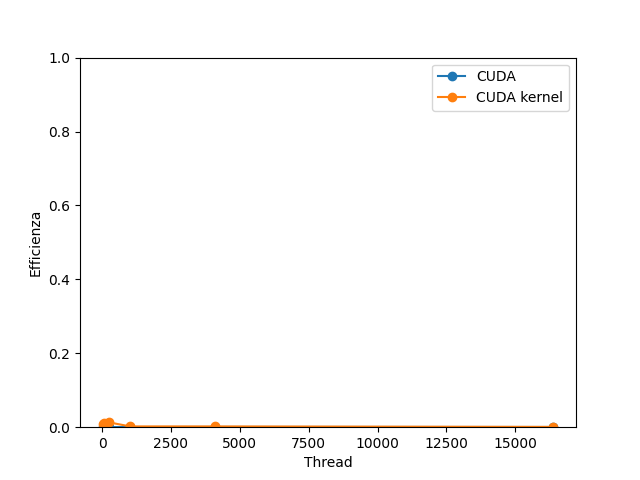
\includegraphics[width=\textwidth]{./imgs/graphs/caso_c_efficiency.png}
        \end{minipage}
    \end{figure}
\end{frame}

\begin{frame}{Analisi}{Test - 4}
    \begin{enumerate}
        \item[4.] Aumentando i processi, a parità di thread (1024) e dimensione del problema \textbf{per thread}
    \end{enumerate}

    \begin{figure}[H]
        \centering
        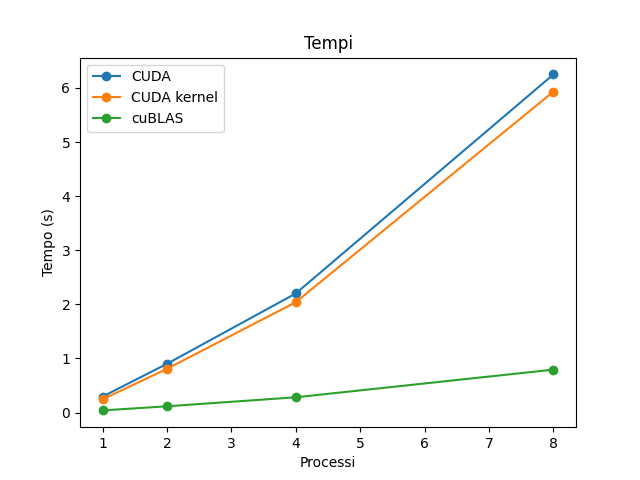
\includegraphics[width=0.6\textwidth]{./imgs/graphs/caso_d.png}
    \end{figure}
\end{frame}

\begin{frame}{Analisi}{Test - 4}
    \begin{figure}[H]
        \centering
        \begin{minipage}{0.48\textwidth}
            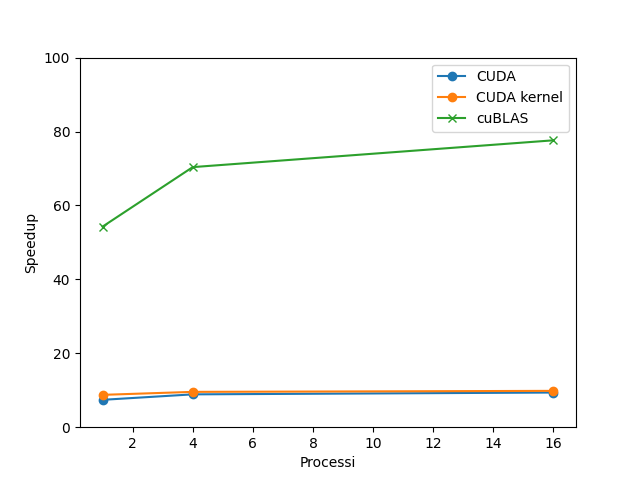
\includegraphics[width=\textwidth]{./imgs/graphs/caso_d_speedup.png}
        \end{minipage}
        \begin{minipage}{0.48\textwidth}
            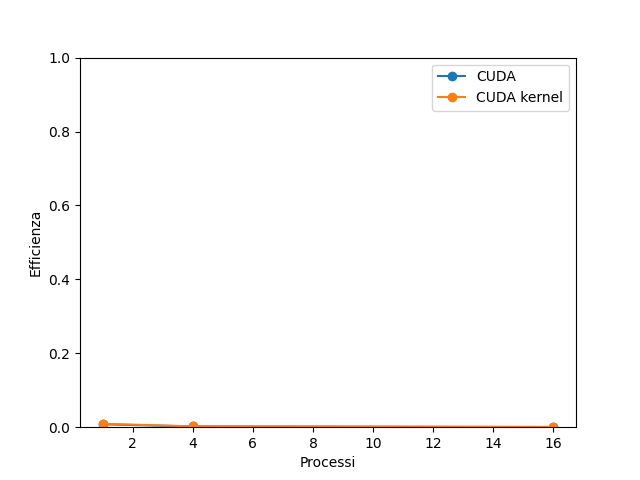
\includegraphics[width=\textwidth]{./imgs/graphs/caso_d_efficiency.png}
        \end{minipage}
    \end{figure}
\end{frame}

\begin{frame}{Analisi}{Conclusioni}
    \begin{itemize}
        \item Non vantaggioso per matrici piccole ($\approx 512 \times 512$)
        \item Aumentare thread più vantaggioso dell'aumentare i processi
              \begin{itemize}
                  \item Tempi di esecuzione minori
                  \item Speedup maggiore
              \end{itemize}
        \item Trasferimento di memoria non tanto un problema...
              \begin{itemize}
                  \item ...ma attesa della stessa GPU da più processi sì
              \end{itemize}
        \item Efficienza quasi nulla
              \begin{itemize}
                  \item Limitazioni della configurazione usata
                  \item Altissimo numero di thread
              \end{itemize}
    \end{itemize}
\end{frame}

\begin{frame}{NCCL - Comunicazione collettiva GPU}
    \begin{itemize}
        \item Libreria NVIDIA per comunicazioni collettive ad alte prestazioni tra GPU.
        \item Supporta ambienti multi-GPU e multi-nodo.
        \item Primitive principali: \texttt{broadcast}, \texttt{reduce}, \texttt{all-reduce}, \texttt{all-gather}, \texttt{reduce-scatter}.
        \item Sfrutta interconnessioni NVLink, PCIe, InfiniBand.
    \end{itemize}
\end{frame}

\begin{frame}{Architettura NCCL}{Comunicazione Peer-to-Peer}
    \begin{itemize}
        \item Comunicazioni dirette GPU-GPU (peer-to-peer), evitando la CPU.
        \item Topologia costruita dinamicamente in fase di inizializzazione.
        \item Supporto per NVLink, PCIe, SHMEM (intra-nodo), UCX (inter-nodo).
        \item Coordinamento tramite topologie a \textbf{ring} e \textbf{albero}.
    \end{itemize}

    \begin{figure}
        \centering
        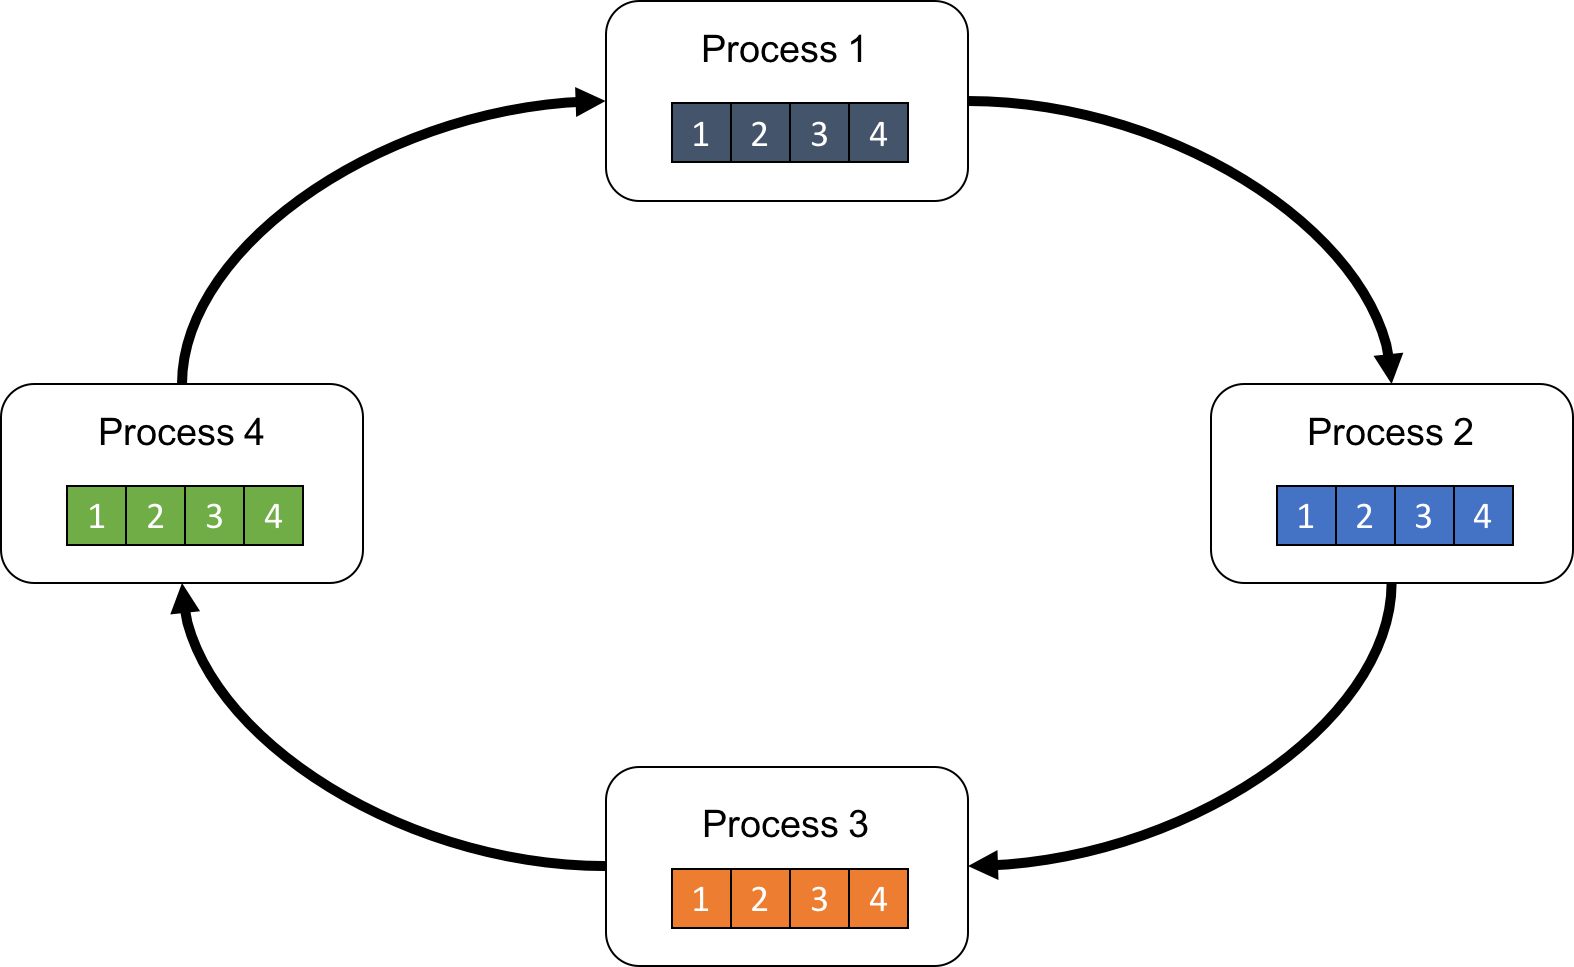
\includegraphics[width=0.48\textwidth]{imgs/nccl_topology_ring_tree.png}%
        \hfill
        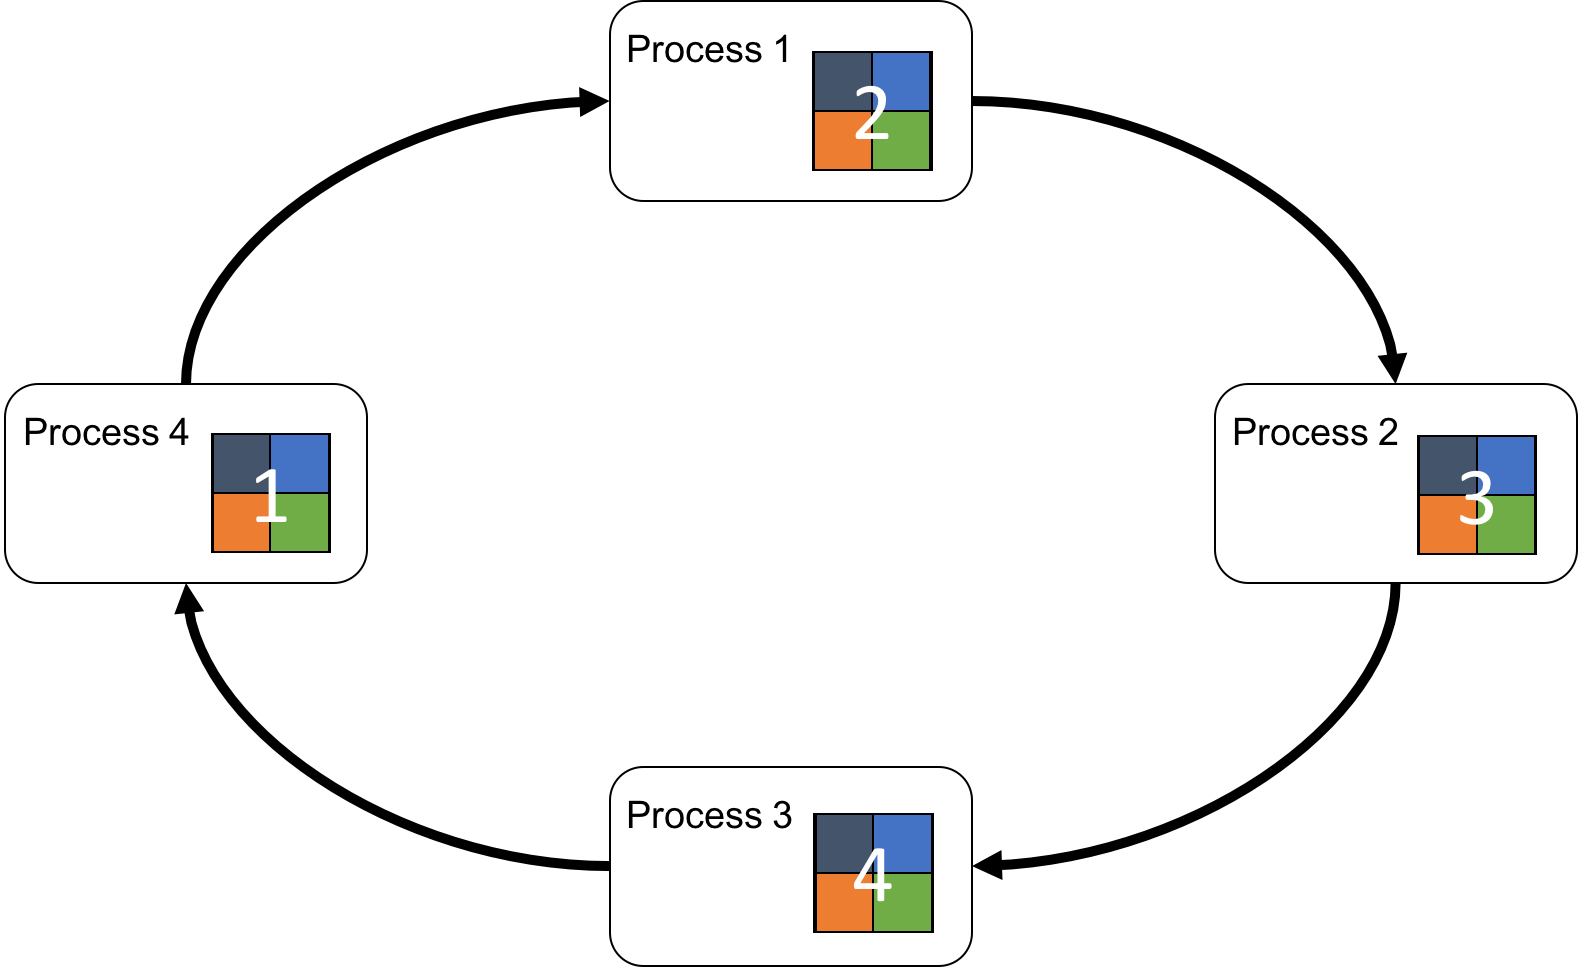
\includegraphics[width=0.48\textwidth]{imgs/nccl_topology_ring_tree_2.png}
        %\caption{Schema topologia ring/allreduce con peer-to-peer}
        \label{fig:ring-tree}
    \end{figure}
\end{frame}

\begin{frame}{Caratteristiche NCCL}{Prestazioni e Asincronicità}
    \begin{itemize}
        \item Comunicazioni asincrone: integrazione con CUDA stream.
        \item Overlapping tra computazione e comunicazione.
        \item Adattamento automatico all’hardware per ridurre latenza e aumentare il throughput.
        \item Ottimizzato per decine o centinaia di GPU.
    \end{itemize}
\end{frame}

\begin{frame}{Confronto con MPI}
    \begin{itemize}
        \item \textbf{Intra-nodo}: NCCL più performante grazie a NVLink e SHMEM.
        \item \textbf{Multi-nodo}: supporta RDMA via UCX/Infiniband.
        \item MPI è più flessibile (comunicazioni punto-a-punto), ma meno ottimizzato per GPU.
        \item NCCL ha un'API più semplice e orientata a CUDA.
    \end{itemize}
\end{frame}

\begin{frame}[fragile]{Esempio NCCL - AllReduce}
    \begin{itemize}
        \item Operazione di \texttt{all-reduce} tra più GPU:
    \end{itemize}

    \begin{lstlisting}[language=C++, basicstyle=\ttfamily\small, keywordstyle=\color{blue}]
        ncclAllReduce(sendbuff, recvbuff, count,
                    ncclFloat, ncclSum,
                    comm, stream);
    \end{lstlisting}

    \begin{itemize}
        \item Comunicazione asincrona rispetto all’host.
        \item \texttt{comm}: comunicatore NCCL. \texttt{stream}: CUDA stream associato.
    \end{itemize}
\end{frame}

\begin{frame}{Limiti e svantaggi}
    \begin{itemize}
        \item Overhead iniziale nella creazione dei comunicatori distribuiti.
        \item Flessibilità limitata: mancano comunicazioni punto-a-punto e topologie arbitrarie.
        \item Supportata solo su GPU NVIDIA e ambienti CUDA.
        \item Ottimale solo con reti ad alte prestazioni (NVLink, InfiniBand).
    \end{itemize}
\end{frame}

\begin{frame}{Applicazione a SUMMA con NCCL}
    \begin{itemize}
        \item NCCL può sostituire \texttt{MPI\_Bcast} per propagare pannelli $\mathbf{A}$ e $\mathbf{B}$.
        \item Due \texttt{ncclBroadcast} paralleli lungo righe e colonne della griglia.
        \item \texttt{ncclGroupStart/End} per gestire sincronizzazione e efficienza.
    \end{itemize}

    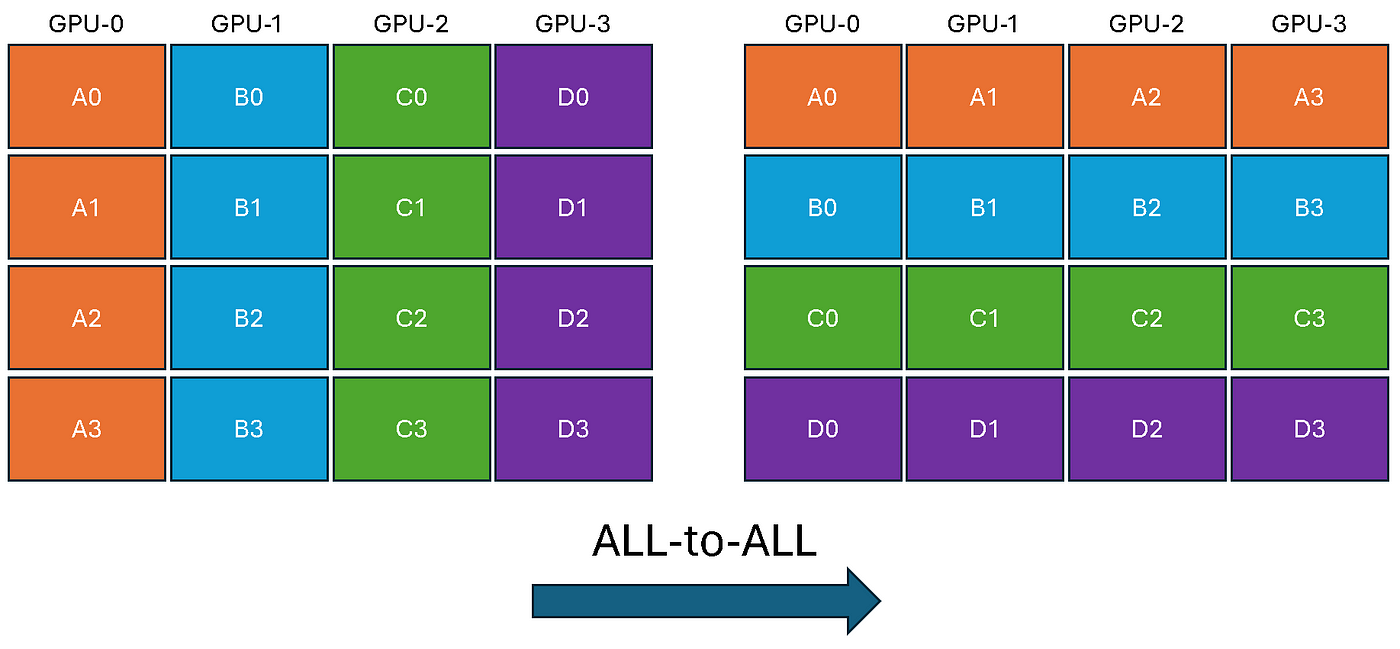
\includegraphics[width=0.6\textwidth]{imgs/summa_nccl.png}
    % Mostrare i due broadcast paralleli nella matrice
\end{frame}

\begin{frame}
    \centering \Huge
    Grazie dell'attenzione
\end{frame}

\end{document}
